%%%%% MOTIVATION & INTRODUCTION
\frame{
\begin{tikzpicture}[remember picture,overlay]
\fill[blue1]
(current page.north west) rectangle ([xshift=0.55\paperwidth,yshift=0.27\paperheight]current page.west|-{pic cs:end});
\end{tikzpicture}
\begin{textblock}{0.55}(0.02,0.03)
	\textcolor{white}{							
	\Large{X-ray radiography of granular systems \\
		-- particle densities and dynamics}
	}
\end{textblock}

\begin{textblock}{0.15}(0.05,0.2)
\includegraphics[width=\textwidth]{Sources/motivation/sand.png}
\\[0.2cm]
\includegraphics[width=\textwidth]{Sources/motivation/coal.png}
\\[0.2cm]
\includegraphics[width=\textwidth]{Sources/motivation/coffee.png}
{\Huge$\vdots$}
\end{textblock}

\begin{textblock}{0.3}(0.3,0.4)
\centering
\visible<4->{
Dissipative interactions\\[0.1cm]
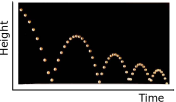
\includegraphics[width=\textwidth]{Sources/motivation/Driscoll_et_al_2016.png}\\
{\scriptsize Driscoll \textit{et al} (2016)}}
\end{textblock}

\begin{textblock}{0.25}(0.7,0.1)
\centering
\visible<2->{
\textbf{Volume fraction} 
\[\Phi = \frac{V_\text{Particles}}{V_\text{Container}}\]}
\only<2>{
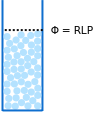
\includegraphics[width=\textwidth]{Sources/motivation/setup-fluidized_bed_sedimented.pdf}}
\only<3,4>{
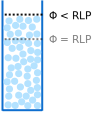
\includegraphics[width=\textwidth]{Sources/motivation/setup-fluidized_bed_expanded.pdf}}
\end{textblock}
}
